%%%%%%%%%%%%%%%%%%%%%%%%%%%%%%%%%%%%%%%%%%%%%%%%%%%%%%%%%%%%%%%%%%%%%%
%%                     Production
%%%%%%%%%%%%%%%%%%%%%%%%%%%%%%%%%%%%%%%%%%%%%%%%%%%%%%%%%%%%%%%%%%%%%%

\subsection{Glyph: \glyph{Production}}\label{sec:production}

\glyph{Production} is the arc used to represent the fact that an entity pool is produced by a process. In the case of a reversible process, the 
\glyph{production} arc also acts as a \glyph{consumption} arc. The target extremity of a \glyph{production} carries a filled arrowhead. A cardinality label can be associated with a \glyph{production} arc indicating the stoichiometry of a process.

\begin{figure}[H]
  \centering
  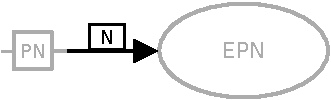
\includegraphics[scale = 0.4]{images/production}
  \caption{The \PD glyph for \glyph{production}.}
  \label{fig:production}
\end{figure}
